\documentclass[12pt,a4paper]{article}

% Overleaf compiler: pdfLaTeX
\usepackage[utf8]{inputenc}
\usepackage[T1]{fontenc}
\usepackage{lmodern}
\usepackage[a4paper,margin=0.85in,headheight=42pt,headsep=18pt,footskip=28pt]{geometry}
\usepackage{amsmath,amssymb}
\usepackage{array,booktabs,tabularx}
\usepackage{enumitem}
\usepackage{fancyhdr}
\usepackage{graphicx}
\usepackage{adjustbox}
\usepackage{microtype}
\usepackage{xcolor}
\usepackage{tikz}
\usepackage[font=small,labelfont=bf]{caption}
\usetikzlibrary{arrows.meta,positioning,calc,shapes.geometric,fit,trees}

\definecolor{navy}{RGB}{31,78,121}
\definecolor{paleBlue}{RGB}{229,237,247}
\definecolor{paleGray}{RGB}{245,246,248}

% Edit this single definition to change the roll number throughout the document.
\newcommand{\RollNumber}{24118105}
\newcommand{\StudentName}{Shourya Veer Singh}

\setlength{\parindent}{0pt}
\setlength{\parskip}{5pt}
\setlist[itemize]{leftmargin=1.5em,itemsep=2pt,topsep=2pt}
\setlist[enumerate]{leftmargin=1.7em,itemsep=2pt,topsep=2pt}
\renewcommand{\arraystretch}{1.2}

\pagestyle{fancy}
\fancyhf{}
\fancyhead[R]{%
  \begin{tabular}{@{}r@{}}
    \small\textbf{Name: \StudentName}\\[-1pt]
    \small Roll No.: \RollNumber\\[-1pt]
    \small Signature: \rule{2.2cm}{0.4pt}
  \end{tabular}}
\fancyfoot[C]{\small ITC Assignment 01}
\fancyfoot[R]{\small\thepage}
\renewcommand{\headrulewidth}{0.4pt}
\renewcommand{\footrulewidth}{0pt}
\fancypagestyle{plain}{%
  \fancyhf{}
  \fancyhead[R]{%
    \begin{tabular}{@{}r@{}}
      \small\textbf{Name: \StudentName}\\[-1pt]
      \small Roll No.: \RollNumber\\[-1pt]
      \small Signature: \rule{2.2cm}{0.4pt}
    \end{tabular}}
  \fancyfoot[C]{\small ITC Assignment 01}
  \fancyfoot[R]{\small\thepage}
  \renewcommand{\headrulewidth}{0.4pt}
}

\tikzset{
  block/.style={draw=navy,fill=paleBlue,rounded corners=2pt,
    minimum height=8mm,text width=24mm,inner sep=1pt,align=center,font=\small},
  smallblock/.style={draw=navy,fill=paleBlue,rounded corners=2pt,
    minimum height=7mm,text width=19mm,inner sep=1pt,align=center,font=\scriptsize},
  sum/.style={draw=navy,circle,minimum size=7mm,inner sep=0pt,font=\small},
  arrow/.style={-{Stealth[length=2mm]},thick,draw=navy},
  link/.style={thick,draw=navy},
  treenode/.style={circle,draw=navy,fill=paleBlue,inner sep=2pt,
    minimum size=7mm,font=\scriptsize,align=center},
  leafnode/.style={rectangle,draw=navy,fill=paleBlue,rounded corners=1pt,
    inner sep=2.5pt,font=\scriptsize,align=center}
}

\newenvironment{scaledtikz}
  {\begin{adjustbox}{width=0.95\linewidth,keepaspectratio}\begin{tikzpicture}}
  {\end{tikzpicture}\end{adjustbox}}
\newcommand{\DiagramStart}{\begin{scaledtikz}}
\newcommand{\qheading}[1]{\section*{#1}}
\newcommand{\topic}[1]{\paragraph{\color{navy}#1.}}

\begin{document}

\begin{titlepage}
\thispagestyle{fancy}
\vspace*{1.2cm}
\begin{center}
{\Large\bfseries NATIONAL INSTITUTE OF TECHNOLOGY RAIPUR\par}
\vspace{0.35cm}
{\large Department of Information Technology\par}
\vspace{1.1cm}
{\LARGE\bfseries ASSIGNMENT 01\par}
\vspace{0.45cm}
{\large Course: ITC\par}
{\large B.Tech. -- Fifth Semester\par}
\vfill
\end{center}
\begin{center}
\renewcommand{\arraystretch}{1.6}
\begin{tabular}{|>{\bfseries}p{4cm}|p{8cm}|}
\hline
Name & \StudentName\\ \hline
Roll Number & \RollNumber\\ \hline
Signature & \rule{5cm}{0.4pt}\\ \hline
\end{tabular}
\end{center}
\vfill
\end{titlepage}

\qheading{Q1. Fundamental Principles of Data Compression}

\topic{Introduction}
Data compression is the process of representing information with fewer bits than the original representation while preserving the required level of information or quality. It is essential because digital data requires storage space, bandwidth, and transmission time. Compression reduces cost and improves communication speed, but it must maintain an acceptable trade-off between size, quality, and computational complexity.

\topic{Need for Data Compression}
Text, images, audio, and video commonly contain large volumes of repeated, correlated, or less important information. Compression supports faster file transfer, efficient use of network bandwidth, smaller backups, economical cloud storage, and quicker loading of multimedia on web and mobile devices.

\topic{Types of Redundancy}
Coding redundancy means that symbols are represented with more bits than necessary. Spatial redundancy occurs when neighbouring image pixels have similar values. Temporal redundancy occurs when consecutive frames in video are nearly identical. Inter-symbol redundancy arises when some symbol combinations occur more frequently or are predictable. Statistical redundancy exists when symbol probabilities are non-uniform.

\topic{Lossless and Lossy Compression}
Lossless compression guarantees exact reconstruction. It is used for text, executable files, source code, medical records, and archival data. Typical techniques include Run-Length Coding, Huffman Coding, Arithmetic Coding, LZW, and dictionary methods. Lossy compression discards information considered less perceptually important. It is used for photographs, audio, and video. JPEG, MPEG, MP3, and AAC are examples. The level of loss is controlled to achieve a desired quality--size trade-off.

\topic{Compression Ratio}
Compression ratio (CR) is usually expressed as
\[
C_R=\frac{\text{original size}}{\text{compressed size}}.
\]
It may also be expressed as percentage saving:
\[
\text{Percentage saving}=100\left(1-\frac{\text{compressed size}}{\text{original size}}\right).
\]
For example, a 100 kB file stored in 25 kB has a compression ratio of 4:1 and saves 75\% of the original storage.

\topic{Coding Efficiency}
Coding efficiency is the ratio of average information content (entropy) to the average code length:
\[
\eta=\frac{H(S)}{L_{\text{avg}}}.
\]
It is close to 100\% when the average code length approaches the entropy. For a symbol source,
\[
H(S)=-\sum_i p_i\log_2 p_i.
\]
It gives the theoretical lower bound on average bits per symbol for a uniquely decodable code.

\topic{Text-Compression Approaches}
Statistical coding assigns shorter codes to frequent symbols and longer codes to rare symbols. Huffman coding constructs a binary tree by repeatedly merging two least-frequent symbols. Arithmetic coding represents an entire message as a fraction in \([0,1)\). Dictionary coding replaces recurring words or phrases with references to a dictionary; LZ77 uses a sliding window and LZ78/LZW build or transmit dictionary entries. Run-length coding is useful for long runs of identical symbols, but is not efficient for ordinary unstructured text without prior preprocessing.

\clearpage
\qheading{Q2. Static Huffman Coding}

\topic{Working Principle}
Static Huffman Coding uses symbol frequencies known before encoding. All symbols are placed in a priority queue ordered by frequency. The two least-frequent nodes are removed and joined as a parent whose weight is their sum. This process continues until one tree remains. The left branch is labelled 0 and the right branch is labelled 1, or vice versa, and the code for a symbol is obtained from the root-to-leaf path.

\topic{Construction}
Initial frequencies are \(E=10\), \(C=15\), \(D=15\), \(B=20\), and \(A=40\). Merge \(E(10)\) and \(D(15)\) to obtain node \(X=25\). Merge \(C(15)\) and \(B(20)\) to obtain \(Y=35\). Merge \(X(25)\) and \(Y(35)\) to obtain \(Z=60\). Finally merge \(Z=60\) with \(A=40\) to obtain root \(=100\).

\topic{Huffman Tree}
\begin{figure}[htbp]
\centering
\resizebox{0.82\linewidth}{!}{%
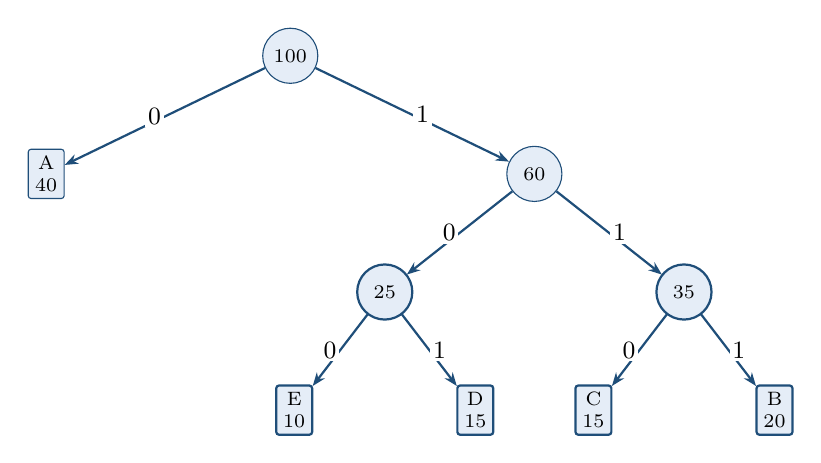
\begin{tikzpicture}[level distance=15mm,
  level 1/.style={sibling distance=62mm},
  level 2/.style={sibling distance=38mm},
  level 3/.style={sibling distance=23mm},
  edge from parent/.style={draw=navy,thick,-{Stealth[length=1.7mm]}},
  every node/.style={font=\small}]
\node[treenode] {100}
  child { node[leafnode] {A\\40}
    edge from parent node[left,draw=none,fill=white,inner sep=1pt] {0} }
  child { node[treenode] {60}
    child { node[treenode] {25}
      child { node[leafnode] {E\\10}
        edge from parent node[left,draw=none,fill=white,inner sep=1pt] {0} }
      child { node[leafnode] {D\\15}
        edge from parent node[right,draw=none,fill=white,inner sep=1pt] {1} }
      edge from parent node[left,draw=none,fill=white,inner sep=1pt] {0} }
    child { node[treenode] {35}
      child { node[leafnode] {C\\15}
        edge from parent node[left,draw=none,fill=white,inner sep=1pt] {0} }
      child { node[leafnode] {B\\20}
        edge from parent node[right,draw=none,fill=white,inner sep=1pt] {1} }
      edge from parent node[right,draw=none,fill=white,inner sep=1pt] {1} }
    edge from parent node[right,draw=none,fill=white,inner sep=1pt] {1} };
\end{tikzpicture}}
\caption{Static Huffman tree for the given symbol frequencies.}
\label{fig:huffman-tree}
\end{figure}
Therefore, the tree shown gives \(A=0\), \(E=100\), \(D=101\), \(C=110\), and \(B=111\). Codes are prefix-free: no codeword is the prefix of another.

\begin{center}
\begin{tabular}{c|c|c|c}
\toprule
Symbol & Frequency & Code & Code length\\
\midrule
A & 40 & 0 & 1\\
B & 20 & 111 & 3\\
C & 15 & 110 & 3\\
D & 15 & 101 & 3\\
E & 10 & 100 & 3\\
\bottomrule
\end{tabular}
\end{center}

\topic{Average Code Length}
\[
\begin{aligned}
L_{\text{avg}}
&=\frac{40}{100}(1)+\frac{20}{100}(3)+\frac{15}{100}(3)
 +\frac{15}{100}(3)+\frac{10}{100}(3)\\
&=0.40+0.60+0.45+0.45+0.30\\
&=2.20\ \text{bits/symbol}.
\end{aligned}
\]

\topic{Total Bits}
The source contains 40 A, 20 B, 15 C, 15 D, and 10 E symbols. Total bits:
\[
40(1)+20(3)+15(3)+15(3)+10(3)=220\ \text{bits}.
\]

\topic{Entropy and Efficiency}
The entropy of this distribution is
\[
H=-\left(0.40\log_2 0.40+0.20\log_2 0.20
+2(0.15\log_2 0.15)+0.10\log_2 0.10\right)
\approx 2.146\ \text{bits/symbol}.
\]
The coding efficiency is \(H/L_{\text{avg}}\approx 2.146/2.20=97.6\%\), so the average length is close to the entropy. The exact codes may vary if equal-weight nodes are merged in a different valid order, but the average length remains the optimum Huffman value.

\clearpage
\qheading{Q3. Dynamic Huffman Coding}

\topic{Concept}
Dynamic, or adaptive, Huffman Coding does not require all source frequencies beforehand. The encoder and decoder begin with an empty or NYT (Not-Yet-Transmitted) symbol set and update the Huffman tree after each symbol. Both sides perform the same update, so the tree remains synchronized.

\topic{Tree Construction and Update}
For the first occurrence of a symbol, the encoder sends the code for NYT and an identifier for the symbol. It then adds the symbol to the tree. For later occurrences, it sends the current code of the symbol. After every symbol, the node weight is increased and the tree is rearranged while satisfying Huffman/numbered-node invariants. A commonly used algorithm is FGK or Vitter.

\begin{figure}[htbp]
\centering
\DiagramStart
\node[block] (find) at (0,0) {Read next symbol\\and find leaf/NYT};
\node[block] (emit) at (3.4,0) {Transmit current\\code (or NYT + symbol)};
\node[block] (inc) at (6.8,0) {Increment weight\\and update tree};
\node[block] (sync) at (10.2,0) {Decoder mirrors\\the same update};
\draw[arrow] (find)--(emit);
\draw[arrow] (emit)--(inc);
\draw[arrow] (inc)--(sync);
\draw[arrow] (sync.south) -- ++(0,-0.65) -| (find.south);
\end{scaledtikz}
\caption{Adaptive Huffman encoding and synchronized decoder update.}
\label{fig:adaptive-huffman}
\end{figure}

\topic{Update Process}
The encoder finds the symbol leaf, increments its weight, and reorders nodes if necessary. Nodes are swapped with a highest-numbered node of the same weight only when permitted, preserving the sibling property. The decoder performs the same operations after receiving and interpreting each symbol.

\topic{Comparison}
Static Huffman coding stores the complete frequency table and initial code tree, and normally performs two passes: frequency collection and encoding. It requires a header carrying the tree/frequencies or previously agreed statistics. Dynamic Huffman coding requires less pre-transmission model information and can adapt to changing symbol patterns, but requires more memory and processing for tree updates and is sensitive to synchronization errors.

\begin{center}
\begin{tabularx}{\linewidth}{>{\bfseries}p{0.22\linewidth}XX}
\toprule
Property & Static Huffman & Dynamic Huffman\\
\midrule
Statistics & Known before encoding & Updated as symbols arrive\\
Passes & Usually frequency pass, then encode & One pass with synchronized updates\\
Side information & Header or agreed model needed & No complete frequency table required initially\\
Adaptation & Does not adapt to changing statistics & Adapts during coding\\
Cost & Simpler tree operation & More memory and update processing\\
\bottomrule
\end{tabularx}
\end{center}

\topic{Applications}
Static coding is suitable for archiving, document compression, and systems with known or stable distributions. Dynamic coding is useful for streaming or files whose symbol statistics are unknown or vary, especially in on-the-fly encoders.

\clearpage
\qheading{Q4. Arithmetic Coding}

\topic{Principle}
Arithmetic coding represents an entire message as a subinterval of \([0,1)\). No individual symbol is assigned a fixed-width code. At each step, the current interval is divided in proportion to symbol probabilities. For symbols \(A,B,C\) with \(A=[0,0.5)\), \(B=[0.5,0.8)\), \(C=[0.8,1.0)\), the code sequence ABCA is processed as follows.

\topic{Interval Calculation}
For a current interval \([L,U)\), let \(W=U-L\), and let the next symbol occupy the cumulative probability range \([L_s,U_s)\). The updated interval is
\[
L'=L+W L_s,\qquad U'=L+W U_s.
\]
\[
\begin{array}{ll}
\text{Start:} & [0,1),\quad \text{width}=1.\\
A: & [0,0.5),\quad \text{width}=0.5.\\
B: & \text{lower}=0.5+0.5(0)=0.5;\quad
      \text{upper}=0.5+0.5(0.3)=0.65,\quad [0.5,0.65).\\
C: & \text{lower}=0.5+0.15(0.8)=0.62;\quad
      \text{upper}=0.5+0.15(1.0)=0.65,\quad [0.62,0.65).\\
A: & \text{lower}=0.62+0.03(0)=0.62;\quad
      \text{upper}=0.62+0.03(0.5)=0.635,\quad [0.62,0.635).
\end{array}
\]
\begin{figure}[htbp]
\centering
\DiagramStart
\draw[link] (0,0)--(10,0);
\foreach \x/\lab in {0/0,5/0.5,8/0.8,10/1.0}
  {\draw[link] (\x,0.08)--(\x,-0.08) node[below=2pt,font=\scriptsize] {\lab};}
\draw[line width=4pt,navy] (0,0.55)--(5,0.55);
\node[above,font=\scriptsize] at (2.5,0.58) {A};
\draw[line width=4pt,red!70!black] (5,1.0)--(6.5,1.0);
\node[above,font=\scriptsize] at (5.75,1.03) {B within A};
\draw[line width=4pt,green!50!black] (6.2,1.45)--(6.5,1.45);
\node[above,font=\scriptsize] at (6.35,1.48) {C};
\draw[line width=4pt,orange!80!black] (6.2,1.9)--(6.35,1.9);
\node[above,font=\scriptsize] at (6.28,1.93) {final A interval};
\draw[dashed] (6.2,0.1)--(6.2,2.1);
\draw[dashed] (6.35,0.1)--(6.35,2.1);
\end{scaledtikz}
\caption{Nested intervals for arithmetic encoding of ABCA.}
\label{fig:arithmetic-intervals}
\end{figure}

\topic{Final Encoded Value}
Choose the midpoint of the final interval:
\[
\frac{0.620+0.635}{2}=0.6275.
\]
The value 0.6275 lies inside \([0.62,0.635)\), so it uniquely identifies ABCA when the symbol probabilities and message length or termination convention are known.

\topic{Comparison with Huffman Coding}
Huffman coding assigns integer-length codes to symbols and is simple to implement. Arithmetic coding approaches the entropy closely even when symbol probabilities do not produce convenient fixed-length Huffman codes, and it can encode the whole sequence into a fractional value. Arithmetic coding is often more storage efficient for very skewed distributions, but it is numerically and computationally more complex. With long sequences, implementation uses finite-precision scaling and renormalization.

\clearpage
\qheading{Q5. Image Compression; GIF and TIFF}

\topic{Need and Basic Principles}
Images contain many pixels and may have spatial redundancy, limited colour variety, or content that the human eye cannot distinguish precisely. Compression reduces storage and transmission costs, speeds loading and printing, and enables archiving of large image collections.

\begin{figure}[htbp]
\centering
\DiagramStart
\node[block] (image) at (0,0) {Image samples\\and redundancy};
\node[block] (analysis) at (3.6,0) {Represent / transform\\and encode};
\node[block] (file) at (7.2,0) {Compressed image\\file};
\node[block] (display) at (10.8,0) {Decode for\\display / print};
\draw[arrow] (image)--(analysis);
\draw[arrow] (analysis)--(file);
\draw[arrow] (file)--(display);
\end{scaledtikz}
\caption{General image compression and reconstruction workflow.}
\label{fig:image-compression}
\end{figure}

\topic{GIF}
Features: GIF is a lossless, indexed-colour raster format using a palette of at most 256 colours. It supports interlacing, transparency, and short animation sequences. It commonly uses LZW dictionary compression. Advantages include wide browser support, small files for flat graphics, simple animation support, and no patent-issue concerns in modern use. Limitations include poor support for high-colour photographs, a fixed 8-bit palette per frame, limited control of compression quality, and larger files for complex real-world images.

\topic{TIFF}
Features: TIFF is a flexible, tagged, high-quality raster format. It can use RGB, greyscale, palette, CMYK, and many bit-depth configurations. It supports multiple pages/layers, metadata, scan data, and lossless methods such as LZW, PackBits, ZIP/Deflate, or none. Some TIFF variants support lossy JPEG compression. Advantages include excellent quality, high bit depth, broad professional and archival use, and strong metadata support. Limitations include very large file sizes, complexity due to many optional extensions, slower processing, and poor suitability for web delivery.

\topic{GIF versus TIFF}
\begin{center}
\begin{tabularx}{\linewidth}{>{\bfseries}p{0.17\linewidth}XX}
\toprule
Property & GIF & TIFF\\
\midrule
Colour/quality & Indexed palette of at most 256 colours & RGB, greyscale, palette, CMYK, and varied bit depths\\
Compression & Commonly LZW; lossless & LZW, PackBits, ZIP/Deflate, none; some variants allow lossy JPEG\\
Capabilities & Interlacing, transparency, short animation & Multiple pages/layers, metadata, scan data\\
Advantages & Browser support, compact flat graphics, simple animation & High quality, fidelity, professional/archival use\\
Limitations & Poor for photographs and complex colour & Large files, many optional extensions, slower processing, poor web fit\\
Typical use & Logos, icons, simple diagrams, memes, animation & Scanning, medical imaging, publishing, print workflows\\
\bottomrule
\end{tabularx}
\end{center}
GIF is mainly appropriate for logos, icons, simple diagrams, memes, and frame-by-frame animations. TIFF is used in document scanning, medical imaging, publishing, and print workflows where fidelity and metadata are important. TIFF provides higher quality and flexibility, while GIF prioritizes simple web-compatible graphics and small animated files.

\clearpage
\qheading{Q6. Digitized Documents}

\topic{Concept}
A digitized document is an electronic representation of a paper document. It may be a raster image, a searchable OCR (Optical Character Recognition) text layer, or a hybrid PDF. Digitization preserves accessibility and allows indexing, transmission, printing, editing, and backup.

\topic{Conversion Process}
The paper is prepared and scanned using a flatbed or sheet-fed scanner. Illumination and acquisition convert light reflected from the page into electrical signals. Sampling creates pixels, quantization assigns intensity levels, and optional colour correction or de-skewing improves the result. OCR then recognizes characters, and PDF or TIFF packages the image and searchable text.

\begin{figure}[htbp]
\centering
\DiagramStart
\node[smallblock] (paper) at (0,0) {Paper page};
\node[smallblock] (scan) at (2.6,0) {Scanner optics\\and sensor};
\node[smallblock] (sample) at (5.2,0) {Sampling and\\quantization};
\node[smallblock] (process) at (7.8,0) {Image cleanup\\and de-skew};
\node[smallblock] (ocr) at (10.4,0) {OCR text layer\\and PDF/TIFF};
\draw[arrow] (paper)--(scan);
\draw[arrow] (scan)--(sample);
\draw[arrow] (sample)--(process);
\draw[arrow] (process)--(ocr);
\end{scaledtikz}
\caption{Paper-document digitization, processing, and OCR workflow.}
\label{fig:document-digitization}
\end{figure}

\topic{Image Acquisition}
A scanner's optical system, sensor, and software determine the quality of acquisition. Clean optics, correct colour settings, flat pages, and controlled lighting reduce noise and shadows.

\topic{Resolution}
Resolution is measured in dots per inch (dpi). 150--300 dpi is typical for office documents, while 600 dpi or more may be used for fine print or archival scanning. Higher resolution captures more detail but increases storage and processing requirements.

\topic{Bit Depth}
Bit depth is the number of bits used for each pixel component. Binary 1-bit depth is suitable for clean black-and-white text, 8 bits per channel is common for greyscale or 256-level colour, and 24-bit colour has 8 bits for each RGB channel. More bit depth improves tonal fidelity but increases size.

\topic{Image Representation}
Text pages may be represented as bilevel or greyscale images. The page may be a bitmap or, after OCR, XML/text. PDF can contain a raster page with an invisible or searchable text layer.

\topic{Compression}
Lossless compression preserves exact pixel values and is used for financial, legal, archival, and OCR-critical documents. TIFF with LZW/ZIP or PDF with lossless image streams are common. Lossy JPEG may be used when controlled quality loss is acceptable; JBIG-type coding is suitable for bilevel document images and is typically lossless. Compression reduces storage and transmission cost, enables faster indexing or download, and supports large document-management repositories.

\clearpage
\qheading{Q7. JPEG Image Compression}

\topic{Principle}
JPEG is a lossy compression standard for continuous-tone grayscale and colour images. It exploits the fact that natural images contain spatial redundancy and that human visual perception is less sensitive to high-frequency spatial detail.

\topic{JPEG Encoder Block Diagram}
\begin{figure}[htbp]
\centering
\DiagramStart
\node[smallblock] (rgb) at (0,0) {Input image\\RGB};
\node[smallblock] (ycc) at (2.25,0) {RGB to\\YCbCr};
\node[smallblock] (blocks) at (4.5,0) {8x8 blocks\\and level shift};
\node[smallblock] (dct) at (6.75,0) {2-D DCT};
\node[smallblock] (quant) at (9,0) {Quantization};
\node[smallblock] (zig) at (11.25,0) {Zigzag, RLE,\\Huffman};
\draw[arrow] (rgb)--(ycc);
\draw[arrow] (ycc)--(blocks);
\draw[arrow] (blocks)--(dct);
\draw[arrow] (dct)--(quant);
\draw[arrow] (quant)--(zig);
\node[font=\scriptsize,below=4mm of zig] {JPEG bitstream};
\end{scaledtikz}
\caption{Baseline JPEG encoder pipeline.}
\label{fig:jpeg-encoder}
\end{figure}

\topic{Color Space Conversion}
The RGB image is transformed to a luminance component \(Y\) and chrominance components \(C_b\) and \(C_r\). Since human vision is more sensitive to luminance, the chrominance planes are often subsampled 4:2:0 or 4:2:2.

\topic{DCT}
Each 8x8 block is transformed from the spatial domain to frequency coefficients using the Discrete Cosine Transform. One coefficient represents the average or DC value, and the remaining coefficients represent increasing spatial frequencies.
For an 8x8 block \(f(x,y)\), the two-dimensional DCT is
\[
F(u,v)=\frac{1}{4}C(u)C(v)
\sum_{x=0}^{7}\sum_{y=0}^{7} f(x,y)
\cos\!\left(\frac{(2x+1)u\pi}{16}\right)\,
\cos\!\left(\frac{(2y+1)v\pi}{16}\right),
\]
where \(0\leq u,v\leq7\), \(C(0)=1/\sqrt{2}\), and \(C(k)=1\) for \(k>0\).
The inverse transform reconstructs the spatial block:
\[
\widehat{f}(x,y)=\frac{1}{4}\sum_{u=0}^{7}\sum_{v=0}^{7}
C(u)C(v)F(u,v)
\cos\!\left(\frac{(2x+1)u\pi}{16}\right)\,
\cos\!\left(\frac{(2y+1)v\pi}{16}\right).
\]

\topic{Quantization}
Each DCT coefficient is divided by a corresponding value in a quantization table and rounded. The larger table values for high frequencies remove fine detail and reduce precision, producing zeros and compression. The quantization table and quality factor control the quality--size trade-off.
If \(Q(u,v)\) is the quantization-table entry, quantization and inverse quantization are
\[
F_q(u,v)=\operatorname{round}\!\left(\frac{F(u,v)}{Q(u,v)}\right),
\qquad
\widehat{F}(u,v)=F_q(u,v)Q(u,v).
\]
Rounding during quantization is the principal lossy step in baseline JPEG.

\topic{Zigzag Scanning}
Coefficients are read in zigzag order from low frequency to high frequency. This tends to place non-zero coefficients first and long runs of zeros later.

\topic{Run-Length Encoding}
Zero coefficients are encoded using run-length pairs (run of zeros, non-zero value). End-of-Block markers indicate that the remaining coefficients in a block are zero.

\topic{Huffman Coding}
Final values and run/amplitude symbols are represented by variable-length Huffman codes. Frequent symbols receive short codes, and rare symbols receive longer codes.

\topic{Lossy versus Lossless}
JPEG baseline mode is lossy. Loss occurs primarily at quantization and cannot be fully recovered. Lossless JPEG modes and formats such as PNG or TIFF with lossless coding allow exact reconstruction of the original pixels.

\clearpage
\qheading{Q8. Differential Pulse Code Modulation (DPCM)}

\topic{Principle}
Pulse Code Modulation encodes each sample independently. DPCM reduces redundancy by encoding only the difference between the actual sample and a prediction of that sample. Adjacent samples in a slowly varying signal are often similar, so the prediction error has a smaller range than the original sample.
For \(b\) bits per sample and sampling frequency \(f_s\), uncompressed PCM has bit rate \(R_{\mathrm{PCM}}=b f_s\). PCM quantizes each sample independently as \(x_q[n]=Q_b(x[n])\).

\topic{DPCM Block Diagram}
\begin{figure}[htbp]
\centering
\DiagramStart
\node[block] (input) at (0,1.6) {Input \(x[n]\)};
\node[sum] (diff) at (2.7,1.6) {\(+/-\)};
\node[block] (quant) at (5.3,1.6) {Error\\quantizer};
\node[block] (enc) at (8,1.6) {Encoder};
\node[block] (channel) at (10.7,1.6) {Bitstream};
\node[block] (decoder) at (13.4,1.6) {Decoder};
\node[sum] (add) at (13.4,-1) {\(+\)};
\node[block] (output) at (10.4,-1) {Reconstructed\\sample};
\node[block] (pred) at (6.2,-1) {Predictor};
\draw[arrow] (input)--(diff);
\draw[arrow] (diff)--node[above,font=\scriptsize] {\(e[n]\)}(quant);
\draw[arrow] (quant)--(enc);
\draw[arrow] (enc)--(channel);
\draw[arrow] (channel)--(decoder);
\draw[arrow] (decoder.south)--(add.north);
\draw[arrow] (add.west)--(output.east);
\draw[arrow] (output.west)--(pred.east);
\draw[arrow] (pred.north) -- ++(0,1.1) -| (diff.south);
\draw[arrow] (pred.south) -- ++(0,-0.65) -| (add.south);
\end{scaledtikz}
\caption{DPCM encoder and decoder with prediction, quantization, reconstruction, and feedback.}
\label{fig:dpcm}
\end{figure}

\topic{Predictor}
The predictor estimates the next sample from previous reconstructed samples. A simple predictor may output \(\hat{x}[n]=\widetilde{x}[n-1]\). In practice, a linear predictor uses several past samples.
More generally,
\[
\hat{x}[n]=\sum_{k=1}^{p}a_k\widetilde{x}[n-k],
\]
where \(\widetilde{x}\) denotes past reconstructed samples.

\topic{Quantizer}
The quantizer maps the prediction error \(e[n]=x[n]-\hat{x}[n]\) to a finite set of levels. This introduces quantization error and determines the output bit rate.
The quantized error and reconstructed sample are
\[
e_q[n]=Q(e[n]),\qquad \widetilde{x}[n]=\hat{x}[n]+e_q[n].
\]

\topic{Encoder}
The encoder converts the quantizer index into a binary word. The receiver uses the same predictor and adds the decoded difference to the predicted value to reconstruct the signal.

\topic{Advantages}
DPCM uses fewer bits per sample than PCM for correlated signals, provides lower bit rate for similar quality, and can be implemented relatively easily.

\topic{Limitations}
It is sensitive to prediction and channel errors, requires feedback or the same reconstructed history at transmitter and receiver, and may suffer poor performance for signals that are difficult to predict.

\clearpage
\qheading{Q9. Adaptive Differential Pulse Code Modulation (ADPCM)}

\topic{Concept}
ADPCM improves DPCM by adapting the quantizer step size and/or predictor to signal characteristics. It therefore works well for both small- and large-amplitude variations.

\topic{ADPCM Block Diagram}
\begin{figure}[htbp]
\centering
\DiagramStart
\node[block] (input) at (0,1.6) {Input \(x[n]\)};
\node[sum] (sub) at (2.7,1.6) {\(+/-\)};
\node[block] (aq) at (5.5,1.6) {Adaptive\\quantizer};
\node[block] (enc) at (8.2,1.6) {Encoder};
\node[block] (bits) at (10.8,1.6) {Bitstream};
\node[block] (decoder) at (13.4,1.6) {Decoder};
\node[sum] (add) at (13.4,-1) {\(+\)};
\node[block] (output) at (10.4,-1) {Reconstructed\\sample};
\node[block] (pred) at (6.2,-1) {Adaptive\\predictor};
\node[block] (adapt) at (2.7,-2.8) {Step-size and\\predictor update};
\draw[arrow] (input)--(sub);
\draw[arrow] (sub)--node[above,font=\scriptsize] {prediction error}(aq);
\draw[arrow] (aq)--(enc);
\draw[arrow] (enc)--(bits);
\draw[arrow] (bits)--(decoder);
\draw[arrow] (decoder.south)--(add.north);
\draw[arrow] (add.west)--(output.east);
\draw[arrow] (output.west)--(pred.east);
\draw[arrow] (pred.north) -- ++(0,1.1) -| (sub.south);
\draw[arrow] (pred.south) -- ++(0,-0.65) -| (add.south);
\draw[arrow] (aq.south) -- ++(0,-4.0) -| (adapt.east);
\draw[arrow] (adapt.north) -- ++(0,1.5) -| (aq.south west);
\end{scaledtikz}
\caption{ADPCM encoder and decoder with synchronized step-size and predictor adaptation.}
\label{fig:adpcm}
\end{figure}

\topic{Adaptation of Step Size}
When successive quantizer indices indicate that the signal is highly varying or the error is large, the step-size adaptation logic increases \(\Delta\). If the signal is slowly varying and errors are small, \(\Delta\) is decreased. Multiplication factors, look-up tables, or recursive adaptation rules are used.
The adaptive quantizer may be expressed as
\[
e_q[n]=Q_{\Delta[n]}(e[n]),\qquad
\Delta[n+1]=F\bigl(\Delta[n],i[n]\bigr),
\]
where \(i[n]\) is the current quantizer index and \(F\) is the adaptation rule shared by encoder and decoder.

\topic{Working}
The current prediction is subtracted from the input. The adaptive quantizer encodes the resulting difference using a dynamically controlled step size. The decoder updates the same step size and predictor to reconstruct the sample.

\topic{PCM, DPCM, and ADPCM Comparison}
PCM encodes each sample independently and has high predictability but a high bit rate. DPCM encodes prediction error and is efficient for correlated signals. ADPCM additionally adapts to signal amplitude and is most efficient in variable speech and audio applications. ADPCM usually has higher complexity than DPCM and PCM, but it gives lower bit rates with better perceived quality.

\begin{center}
\begin{tabularx}{\linewidth}{>{\bfseries}p{0.18\linewidth}XXX}
\toprule
Method & What is encoded & Main advantage & Main trade-off\\
\midrule
PCM & Each sample independently & Simple, predictable reconstruction & Higher bit rate\\
DPCM & Difference from predicted sample & Efficient for correlated signals & Depends on predictor and reconstructed history\\
ADPCM & Adaptively quantized prediction error & Better handling of changing signal amplitude; lower bit rates with good perceived quality & More adaptation logic and synchronization\\
\bottomrule
\end{tabularx}
\end{center}

\clearpage
\qheading{Q10. Adaptive Subband Coding}

\topic{Concept}
Subband coding divides an audio signal into several frequency bands, typically using analysis filter banks. Each band is coded independently according to its signal power and perceptual importance.

\topic{Division into Subbands}
A low-pass/high-pass quadrature mirror filter bank or a related filter bank separates the input. Repeated filtering and downsampling create low, mid, and high-frequency bands. The bands are approximately orthogonal or can be reconstructed by a synthesis filter bank.

\topic{Adaptive Subband Coding Diagram}
\begin{figure}[htbp]
\centering
\DiagramStart
\node[block] (input) at (0,0) {Audio input};
\node[block] (analysis) at (3,0) {Analysis filter\\bank};
\node[smallblock] (low) at (6,1.5) {Low-frequency\\subband};
\node[smallblock] (mid) at (6,0) {Mid-frequency\\subband};
\node[smallblock] (high) at (6,-1.5) {High-frequency\\subband};
\node[smallblock] (q1) at (9,1.5) {Adaptive\\quantizer};
\node[smallblock] (q2) at (9,0) {Adaptive\\quantizer};
\node[smallblock] (q3) at (9,-1.5) {Adaptive\\quantizer};
\node[block] (mux) at (12,0) {Bit allocation\\and bitstream};
\draw[arrow] (input)--(analysis);
\draw[arrow] (analysis)--(low);
\draw[arrow] (analysis)--(mid);
\draw[arrow] (analysis)--(high);
\draw[arrow] (low)--(q1);
\draw[arrow] (mid)--(q2);
\draw[arrow] (high)--(q3);
\draw[arrow] (q1)--(mux);
\draw[arrow] (q2)--(mux);
\draw[arrow] (q3)--(mux);
\node[font=\scriptsize,align=center] at (9,-2.5) {Subband energy and psychoacoustic masking\\control quantizer step sizes and allocated bits};
\end{scaledtikz}
\caption{Adaptive subband analysis and independent band coding.}
\label{fig:adaptive-subband}
\end{figure}

\topic{Independent Encoding}
Each subband is sampled at a rate appropriate to its bandwidth and may use PCM or ADPCM coding. High-energy bands and perceptually important bands receive more bits.

\topic{Adaptive Bit Allocation}
The encoder estimates the energy, spectral content, and masking level of each band. It allocates bits according to a distortion criterion and perceptual weighting. Bands with little power or already masked content receive fewer or zero bits.

\topic{Advantages}
Subband coding separates unlike frequency characteristics, reduces quantization noise in low-energy bands, supports efficient adaptive allocation, and can be combined with psychoacoustic masking. It offers better quality than a simple wideband coder at the same bit rate.

\topic{Applications}
It is used in speech and audio compression, including MPEG audio and digital broadcasting, especially where quality and low bit rate are important.

\clearpage
\qheading{Q11. Delta Modulation}

\topic{Principle}
Delta Modulation represents a signal using only 1 bit per sample. The transmitter compares the input sample with a predicted/reconstructed sample and sends 1 if the input is greater and 0 if it is smaller. The step size \(\Delta\) determines the reconstruction change.
For sampling interval \(T_s\), a simple DM encoder and accumulator can be described by
\[
e[n]=x[n]-\widetilde{x}[n-1],\qquad
b[n]=
\begin{cases}
1,&e[n]\geq 0,\\
0,&e[n]<0,
\end{cases}
\]
\[
\widetilde{x}[n]=\widetilde{x}[n-1]+(2b[n]-1)\Delta.
\]

\topic{Delta Modulation Block Diagram}
\begin{figure}[htbp]
\centering
\DiagramStart
\node[block] (input) at (0,1.4) {Input \(x[n]\)};
\node[sum] (cmp) at (3,1.4) {\(+/-\)};
\node[block] (quant) at (5.7,1.4) {1-bit\\quantizer};
\node[block] (bits) at (8.5,1.4) {Bitstream};
\node[block] (acc) at (5.7,-1) {Accumulator\\\(+\Delta/-\Delta\)};
\node[block] (stair) at (9,-1) {Staircase\\estimate};
\draw[arrow] (input)--(cmp);
\draw[arrow] (cmp)--node[above,font=\scriptsize] {error}(quant);
\draw[arrow] (quant)--(bits);
\draw[arrow] (quant.south)--(acc.north);
\draw[arrow] (acc)--(stair);
\draw[arrow] (stair.north) -- ++(0,0.45) -| (cmp.south);
\end{scaledtikz}
\caption{One-bit delta modulator with staircase reconstruction feedback.}
\label{fig:delta-modulation}
\end{figure}

\topic{Working}
The accumulator adds \(+\Delta\) or \(-\Delta\) according to the received bit. The resulting staircase waveform tracks a slowly changing input. The quantization error is the difference between the input and staircase approximation.

\topic{Slope Overload Distortion}
If the input changes faster than the accumulator can follow, the waveform accumulates only \(+\Delta\) or \(-\Delta\) repeatedly and falls behind. This produces slope overload distortion.
For a fixed step size, tracking is limited approximately by the largest step change per sampling interval, \(\Delta/T_s\). A rapidly changing input can exceed this tracking slope.

\topic{Granular Noise}
If \(\Delta\) is much larger than the small variations of a slowly varying signal, the staircase oscillates around the input. This produces granular noise.
Thus, increasing \(\Delta\) helps track steep slopes but can increase granular noise in slowly varying regions.

\topic{Adaptive Delta Modulation}
ADM changes \(\Delta\) according to the bit pattern or signal slope. If several consecutive bits have the same direction, \(\Delta\) increases to follow rapid changes and reduce slope overload. If the direction alternates or changes indicate a slow segment, \(\Delta\) decreases to reduce granular noise.
One illustrative adaptation rule is
\[
\Delta[n+1]=
\begin{cases}
\alpha\Delta[n],&\text{for a run of same-direction bits},\\
\beta\Delta[n],&\text{for alternating bits},
\end{cases}
\qquad \alpha>1,\quad 0<\beta<1.
\]
Practical ADM systems use bounded step sizes and a specified bit-pattern update table.

\begin{figure}[htbp]
\centering
\DiagramStart
\node[block] (bits) at (0,0) {Recent output\\bit pattern};
\node[block] (adapt) at (4,0) {Step-size\\adaptation logic};
\node[block] (delta) at (8,0) {Adaptive\\\(\Delta[n]\)};
\node[block] (acc) at (12,0) {Accumulator\\and estimate};
\draw[arrow] (bits)--(adapt);
\draw[arrow] (adapt)--(delta);
\draw[arrow] (delta)--(acc);
\node[font=\scriptsize,align=center,text width=5cm] at (6,-1.0) {Repeated same-direction bits increase \(\Delta\); alternating bits decrease \(\Delta\).};
\end{scaledtikz}
\caption{Adaptive delta modulation step-size control.}
\label{fig:adaptive-delta}
\end{figure}

\topic{DM versus ADM}
DM uses a fixed step size, is simple, and has 1-bit encoding, but is sensitive to both overload and granular noise. ADM adapts the step size, usually provides better signal-to-noise ratio and can cover more input ranges, but requires more logic and synchronized step-size adaptation.

\clearpage
\qheading{Q12. Low-Bit-Rate Speech Coding and Vocoders}

\topic{Challenges}
Speech varies rapidly in time and frequency and is strongly speaker dependent. Low bit rates must remove not only waveform redundancy but also predictable spectral structure. The coder must preserve intelligibility and naturalness, handle background noise, avoid pitch and timing errors, and remain robust to packet loss.

\topic{Vocoder Principle}
A vocoder models speech production instead of waveform values. It typically separates an excitation source (voiced pulse train or unvoiced noise) from a spectral/vocal-tract filter. Parameters are extracted and transmitted at frame intervals.

\topic{Vocoder Analysis and Synthesis Diagram}
\begin{figure}[htbp]
\centering
\DiagramStart
\node[block] (speech) at (0,1.2) {Speech input};
\node[smallblock] (frame) at (2.6,1.2) {Frame\\windowing};
\node[smallblock] (analysis) at (5.2,1.2) {Pitch/voicing\\and spectral analysis};
\node[smallblock] (params) at (7.9,1.2) {Parameter\\encoder};
\node[smallblock] (bits) at (10.6,1.2) {Bitstream};
\node[smallblock] (decode) at (2.6,-1.2) {Parameter\\decoder};
\node[smallblock] (excite) at (5.2,-1.2) {Pulse/noise\\excitation};
\node[smallblock] (filter) at (7.9,-1.2) {Vocal-tract\\synthesis filter};
\node[block] (out) at (10.6,-1.2) {Reconstructed\\speech};
\draw[arrow] (speech)--(frame);
\draw[arrow] (frame)--(analysis);
\draw[arrow] (analysis)--(params);
\draw[arrow] (params)--(bits);
\draw[arrow] (bits.south) -- ++(0,-0.9) -| (decode.south);
\draw[arrow] (decode)--(excite);
\draw[arrow] (excite)--(filter);
\draw[arrow] (filter)--(out);
\draw[arrow,dashed] (decode.south) -- ++(0,-0.5) -| node[pos=0.7,below,font=\scriptsize] {spectral parameters} (filter.south);
\end{scaledtikz}
\caption{Analysis and synthesis stages of a low-bit-rate vocoder.}
\label{fig:vocoder}
\end{figure}

\topic{Operation}
The analysis stage divides speech into frames, estimates pitch or voicing, computes filter coefficients or an equivalent spectral representation, and estimates gain. The synthesizer recreates voiced excitation or noise and passes it through the vocal-tract filter.

\topic{Applications}
Low-bit-rate vocoders are used in mobile telephony, secure communications, satellite links, military radio, voice storage, and bandwidth-limited networks.

\topic{Limitations}
They may produce robotic or buzzy speech, can lose fine speaker identity, perform poorly in noisy environments, and can be sensitive to frame loss. Naturalness is often lower than waveform coders.

\clearpage
\qheading{Q13. Linear Predictive Coding and CELP}

\topic{LPC Principle}
LPC assumes that each speech sample can be approximated by a linear combination of previous samples. The vocal tract is represented by an all-pole filter. LPC analysis estimates coefficients that minimize the prediction residual.
With predictor order \(p\), one common sign convention is
\[
\widehat{s}[n]=\sum_{k=1}^{p}a_k s[n-k],\qquad
e[n]=s[n]-\widehat{s}[n].
\]
The corresponding synthesis filter is
\[
H(z)=\frac{1}{1-\sum_{k=1}^{p}a_k z^{-k}},
\]
with coefficient signs depending on the predictor convention.

\topic{LPC Analysis}
Speech is divided into overlapping frames and windowed. An autocorrelation or covariance method computes predictor coefficients. A frame gain and pitch/voicing parameters may also be estimated. The residual is the error or excitation that drives the vocal-tract model.

\topic{LPC Synthesis}
At the decoder, the excitation source is generated by a periodic pulse train for voiced speech or noise for unvoiced speech. It is filtered by the LPC synthesis filter to produce speech.

\topic{LPC Analysis and Synthesis Diagram}
\begin{figure}[htbp]
\centering
\DiagramStart
\node[block] (speech) at (0,1.2) {Input speech};
\node[smallblock] (window) at (2.7,1.2) {Frame and\\window};
\node[smallblock] (lpc) at (5.5,1.2) {LPC coefficient\\analysis};
\node[smallblock] (params) at (8.3,1.2) {Coefficients,\\gain, pitch};
\node[block] (bits) at (11.1,1.2) {Encoded\\parameters};
\node[smallblock] (decode) at (2.7,-1.2) {Parameter\\decoder};
\node[smallblock] (excite) at (5.5,-1.2) {Voiced pulse /\\unvoiced noise};
\node[smallblock] (filter) at (8.3,-1.2) {LPC synthesis\\filter};
\node[block] (out) at (11.1,-1.2) {Output speech};
\draw[arrow] (speech)--(window);
\draw[arrow] (window)--(lpc);
\draw[arrow] (lpc)--(params);
\draw[arrow] (params)--(bits);
\draw[arrow] (bits.south) -- ++(0,-0.9) -| (decode.south);
\draw[arrow] (decode)--(excite);
\draw[arrow] (excite)--(filter);
\draw[arrow] (filter)--(out);
\draw[arrow,dashed] (decode.south) -- ++(0,-0.5) -| node[pos=0.7,below,font=\scriptsize] {LPC coefficients} (filter.south);
\end{scaledtikz}
\caption{LPC frame analysis, parameter coding, and synthesis.}
\label{fig:lpc}
\end{figure}

\topic{CELP}
Code Excited Linear Prediction uses LPC synthesis filters but improves excitation through a codebook of candidate excitation vectors. It performs an analysis-by-synthesis search: candidate vectors are filtered and compared with the original speech, and the best codebook index and gain are transmitted.

\begin{figure}[htbp]
\centering
\DiagramStart
\node[block] (target) at (0,0) {Target speech};
\node[block] (search) at (3.5,0) {Search adaptive /\\fixed excitation codebooks};
\node[block] (synth) at (7.2,0) {LPC synthesis\\filter};
\node[block] (compare) at (10.9,0) {Perceptually weighted\\error comparison};
\draw[arrow] (target)--(search);
\draw[arrow] (search)--node[above,font=\scriptsize] {candidate}(synth);
\draw[arrow] (synth)--(compare);
\draw[arrow] (compare.south) -- ++(0,-0.7) -| node[pos=0.25,below,font=\scriptsize] {select best index and gain}(search.south);
\end{scaledtikz}
\caption{CELP analysis-by-synthesis codebook search.}
\label{fig:celp}
\end{figure}

\topic{CELP Improvement}
CELP improves naturalness and reduces buzziness because it represents both periodic and noise-like details through adaptive and fixed codebook excitation. It can capture a wider range of speech events than simple pitch/noise excitation.

\topic{LPC versus CELP}
Traditional LPC coding is less complex and has lower delay, but uses approximate excitation and can sound less natural. CELP provides substantially better quality and lower perceived distortion, but requires codebook search, more computation, more storage, and sometimes higher bit rate.

\clearpage
\qheading{Q14. Perceptual Audio Coding}

\topic{Principle}
Perceptual coding removes or reduces components that are inaudible or less noticeable to a human listener. The encoder uses psychoacoustic models instead of treating all quantization errors equally.

\topic{Frequency Masking}
A strong tone or narrow-band sound makes neighbouring frequencies inaudible. A masker can hide weaker spectral components located close in frequency. The encoder allocates no or very few bits to frequency bins below the masking threshold.

\topic{Temporal Masking}
A strong sound can mask weaker sounds immediately before and after it. Pre-masking is short, while post-masking lasts longer. Temporal masking allows selected samples or transform coefficients to be coded with higher noise.

\topic{Perceptual Audio Coding Diagram}
\begin{figure}[htbp]
\centering
\DiagramStart
\node[block] (audio) at (0,0) {Audio input};
\node[smallblock] (filter) at (2.6,0) {Subband / transform\\filter bank};
\node[smallblock] (psy) at (5.4,1.5) {Psychoacoustic\\masking model};
\node[smallblock] (quant) at (5.4,-0.3) {Quantization and\\bit allocation};
\node[smallblock] (entropy) at (8.4,-0.3) {Entropy coding\\(e.g. Huffman)};
\node[block] (stream) at (11.2,-0.3) {Compressed\\audio bitstream};
\draw[arrow] (audio)--(filter);
\draw[arrow] (filter)--(psy);
\draw[arrow] (filter)--(quant);
\draw[arrow] (psy)--node[right,font=\scriptsize] {masking threshold}(quant);
\draw[arrow] (quant)--(entropy);
\draw[arrow] (entropy)--(stream);
\end{scaledtikz}
\caption{Perceptual audio encoder with masking-based bit allocation.}
\label{fig:perceptual-audio}
\end{figure}

\topic{MPEG Audio}
MPEG audio uses subband or hybrid transform coding, psychoacoustic masking, MDCT-like transforms in later layers, block selection, and Huffman coding. MPEG Layer I, II, and III (MP3) provide increasing efficiency and complexity. MP3 separates frequencies, allocates bits according to masking, and uses Huffman entropy coding.

\topic{Dolby Audio}
Dolby audio systems use perceptual coding, subband or transform filtering, psychoacoustic masking, and proprietary or standardized metadata and processing. Dolby Digital (AC-3) and modern Dolby formats may include multichannel coding and dialog, dynamic-range, or surround metadata.

\topic{Comparison}
MPEG audio is an international, widely interoperable family of perceptual standards used in media, streaming, broadcasting, and digital video. Dolby systems are often optimized for consumer and cinema multichannel experiences and may use proprietary metadata and delivery tools. Both rely on masking and scale-factor/bit-allocation techniques. MPEG MP3 is widely used for general stereo music, while Dolby systems are prominent in film, television, and surround sound.

\begin{center}
\begin{tabularx}{\linewidth}{>{\bfseries}p{0.2\linewidth}XX}
\toprule
Aspect & MPEG audio & Dolby audio\\
\midrule
Coding approach & Subband/hybrid transform, masking, bit allocation, entropy coding & Perceptual subband/transform coding, masking, metadata and processing\\
Examples/use & Layers I, II, III (MP3); streaming, media, broadcasting & Dolby Digital (AC-3) and modern formats; film, TV, multichannel surround\\
Strength & International, widely interoperable family; MP3 is common for stereo music & Often optimized for cinema/consumer multichannel experience\\
\bottomrule
\end{tabularx}
\end{center}

\clearpage
\qheading{Q15. Video Compression; H.261 and MPEG}

\topic{Fundamental Principles}
Video contains spatial redundancy within frames and temporal redundancy between frames. The codec exploits repeated textures, similar neighboring pixels, moving objects, and stationary backgrounds to reduce representation size.

\topic{Spatial and Temporal Redundancy}
Spatial redundancy arises because neighbouring pixels and macroblocks are often similar. Transform coding, quantization, and entropy coding exploit it. Temporal redundancy means consecutive frames contain similar regions. Motion estimation and compensation exploit this redundancy.

\topic{Motion Estimation}
The encoder compares macroblocks or regions in a current frame with candidate regions in a reference frame. A motion vector indicates the best displacement. Metrics such as mean absolute difference or sum of absolute difference are often used.

\topic{Motion Compensation}
The predicted block is reconstructed by shifting the matching block from the reference frame using the motion vector. The encoder stores motion vectors and the residual difference rather than all original pixels.
For a previous reference frame \(F_{t-1}\), motion vector \((u,v)\), and current frame \(F_t\), a typical block predictor and residual are
\[
\widehat{F}_t(x,y)=F_{t-1}(x+u,y+v),\qquad
R_t(x,y)=F_t(x,y)-\widehat{F}_t(x,y).
\]
The decoder reconstructs \(\widetilde{F}_t=\widehat{F}_t+\widetilde{R}_t\), where \(\widetilde{R}_t\) is the decoded residual. B-frame prediction may combine motion-compensated blocks from past and future reference frames.
For example, a bidirectional predictor can be written as
\[
\widehat{F}^{\,B}_t(x,y)=
\alpha F_{t-1}(x+u_1,y+v_1)
+(1-\alpha)F_{t+1}(x+u_2,y+v_2),
\qquad 0\leq\alpha\leq1,
\]
where the two motion vectors point to the past and future reference blocks.

\begin{figure}[htbp]
\centering
\DiagramStart
\node[block] (current) at (0,1.2) {Current frame};
\node[smallblock] (me) at (3,1.2) {Motion\\estimation};
\node[smallblock] (mc) at (6,1.2) {Motion\\compensation};
\node[smallblock] (res) at (9,1.2) {Residual transform,\\quantize, encode};
\node[block] (bits) at (12,1.2) {Video\\bitstream};
\node[block] (ref) at (3,-1.2) {Reference\\frame};
\node[smallblock] (mv) at (6,-1.2) {Motion vectors\\and prediction};
\node[smallblock] (recon) at (9,-1.2) {Reconstructed\\reference frame};
\draw[arrow] (current)--(me);
\draw[arrow] (me)--(mc);
\draw[arrow] (mc)--(res);
\draw[arrow] (res)--(bits);
\draw[arrow] (ref)--(me);
\draw[arrow] (me.south)--(mv.north);
\draw[arrow] (me.north) -- ++(0,0.55) -| node[pos=0.75,above,font=\scriptsize] {motion vectors} (bits.north);
\draw[arrow] (mv)--(recon);
\draw[arrow] (recon.west) -- ++(-0.45,0) |- (ref.south);
\end{scaledtikz}
\caption{Motion estimation, motion compensation, residual coding, and reference reconstruction.}
\label{fig:video-motion}
\end{figure}

\topic{Frame Prediction}
Intra-frame prediction encodes a frame independently. Inter-frame prediction uses one or more previously decoded or future frames to estimate the current frame.

\topic{I-Frames}
I-frames are intra-coded frames. They do not use motion prediction from other frames and provide random-access points. They usually offer the highest size and best decode independence.

\topic{P-Frames}
P-frames are predicted from a previous reference frame. They store motion vectors and residuals and are smaller than I-frames when prediction is accurate.

\topic{B-Frames}
B-frames use both previous and future reference frames for bidirectional prediction. They can achieve greater compression but require frame reordering and additional delay.

\begin{figure}[htbp]
\centering
\resizebox{0.9\linewidth}{!}{%
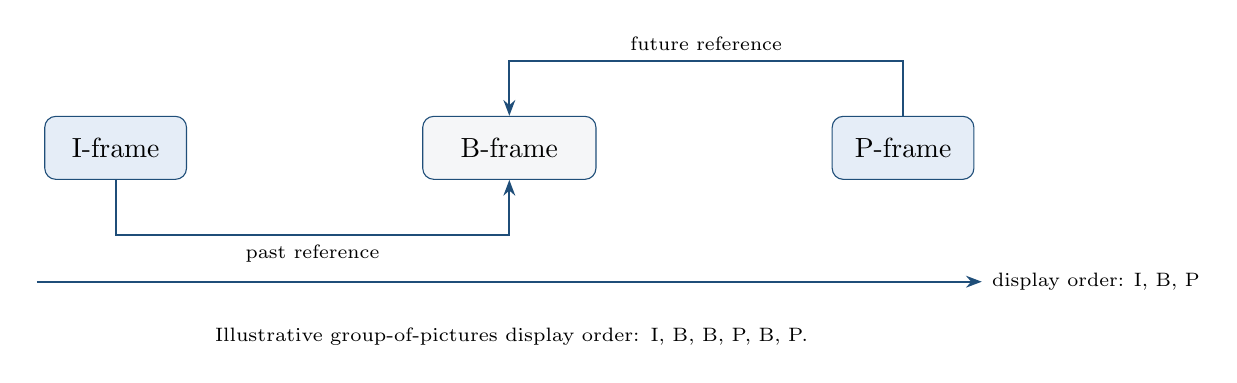
\begin{tikzpicture}[x=1cm,y=1cm]
\node[draw=navy,fill=paleBlue,rounded corners,minimum width=18mm,minimum height=8mm] (iframe) at (0,0) {I-frame};
\node[draw=navy,fill=paleGray,rounded corners,minimum width=22mm,minimum height=8mm] (bframe) at (5,0) {B-frame};
\node[draw=navy,fill=paleBlue,rounded corners,minimum width=18mm,minimum height=8mm] (pframe) at (10,0) {P-frame};
\draw[arrow] (iframe.south) -- ++(0,-0.7) -| node[pos=0.25,below,font=\scriptsize] {past reference} (bframe.south);
\draw[arrow] (pframe.north) -- ++(0,0.7) -| node[pos=0.25,above,font=\scriptsize] {future reference} (bframe.north);
\draw[arrow] (-1,-1.7)--(11,-1.7) node[right,font=\scriptsize] {display order: I, B, P};
\node[font=\scriptsize,align=center,text width=12cm] at (5,-2.4) {Illustrative group-of-pictures display order: I, B, B, P, B, P.};
\end{tikzpicture}}
\caption{B-frame prediction uses both a past I-frame and a future P-frame reference.}
\label{fig:ipb-reference}
\end{figure}

\topic{H.261}
H.261 was designed for videoconferencing at approximately \(p\times64\) kbit/s. It uses CIF/QCIF video, 8x8 DCT blocks, macroblocks, motion compensation, quantization, run-length coding, and variable-length coding. It mainly targets low delay and supports I- and P-frames.

\topic{MPEG}
MPEG standards target stored and broadcast digital video. MPEG-1 was used for CD-quality video, MPEG-2 for DVDs and television broadcasting, and MPEG-4/H.264/HEVC and later variants support more resolutions, coding tools, and lower bit rates. MPEG introduces I-, P-, and B-frame coding, scalable GOP structures, bidirectional prediction, and sophisticated motion compensation.

\topic{H.261 versus MPEG}
H.261 emphasizes low-delay conversational video and simpler prediction, while MPEG emphasizes storage or broadcast efficiency and may use bidirectional B-frames, flexible GOP structures, and higher compression. MPEG systems generally provide better compression and quality for a given application, but can introduce delay and decoder complexity.

\begin{center}
\begin{tabularx}{\linewidth}{>{\bfseries}p{0.2\linewidth}XX}
\toprule
Aspect & H.261 & MPEG family\\
\midrule
Target & Low-delay videoconferencing & Storage, broadcast, and varied resolutions/applications\\
Rates/use & Approximately \(p\times64\) kbit/s; CIF/QCIF & MPEG-1 for CD-quality video; MPEG-2 for DVD/TV; later MPEG-4/H.264/HEVC and successors\\
Tools & 8x8 DCT, macroblocks, motion compensation, quantization, RLE, variable-length coding; I/P prediction & I/P/B frames, flexible/scalable GOP, bidirectional prediction, advanced motion compensation\\
Trade-off & Simpler prediction and low delay & Generally higher compression/quality potential; potentially more delay and decoder complexity\\
\bottomrule
\end{tabularx}
\end{center}

\end{document}
